\documentclass[aspectratio=1610,14pt,t]{beamer}

% Colors
\usepackage{color}
\definecolor{mainorange}{HTML}{EC811B}
\definecolor{lightgrey}{HTML}{888888}
\definecolor{almostwhite}{HTML}{FEFEFE}

% Syntax highlighting
\usepackage{minted}
\usepackage{alltt}
\newcommand\hi[1]{{\color{mainorange} \textbf{#1}}}

% Custom unicode symbols
\usepackage{newunicodechar}
\newcommand\Warning{%
 \makebox[1.4em][c]{%
 \makebox[0pt][c]{\raisebox{.1em}{\small!}}%
 \makebox[0pt][c]{\color{red}\Large$\bigtriangleup$}}}%

\newunicodechar{⚠}{\Warning}

% Theme
\usetheme[%
  subsectionpage=progressbar,
  numbering=fraction,
  progressbar=foot,
]{metropolis}

% Customization
\usepackage{pagecolor}
\setbeamertemplate{section in toc}[sections numbered]
\setbeamerfont{title}{size=\fontsize{30}{30}}
\setbeamerfont{block title}{size=\large}
\newcommand\sep{\textcolor{lightgrey}{\rule{\linewidth}{0.05mm}}}

% Positioning
% https://tex.stackexchange.com/a/34929/13059
\def\Put(#1,#2)#3{\leavevmode\makebox(0,0){\put(#1,#2){#3}}}

% Meta
\title{Embedded Rust}
\date{2018-01-30}
\author{Raphael Nestler (@rnestler)}
\institute{Rust Zürichsee Meetup}

\begin{document}

\pgfdeclareimage[width=\paperwidth]{bg}{background-dark.pdf}
\pagecolor{almostwhite}  % Prevent speakerdeck from optimizing away the bg color
\usebackgroundtemplate{\pgfuseimage{bg}}
\maketitle

% ----------------------------------------------------------------- %

\begin{frame}[c]{println!("{:?}", Self)}
  Hi! I'm Raphael (@rnestler).

  \pause I live in Rapperswil

  \pause I work at Sensirion ({\small \url{https://sensirion.com}}).

  \pause I'm a founding member of Coredump\\hackerspace ({\small \url{https://coredump.ch}}).
\end{frame}

% ----------------------------------------------------------------- %

\begin{frame}[plain,noframenumbering]
  \frametitle{Outline}
  \setcounter{tocdepth}{1}
  \tableofcontents
\end{frame}

% ----------------------------------------------------------------- %

\pgfdeclareimage[width=\paperwidth]{bg}{background-light.pdf}
\usebackgroundtemplate{\pgfuseimage{bg}}

\section{Embedded Programming}

\begin{frame}[c]{What is an \emph{Embedded System}?}
  \begin{quote}
    A combination of computer hardware and software, and perhaps
    additional mechanical or other parts, designed to perform a dedicated
    function.
  \end{quote}
  Michael Barr. ``Embedded Systems Glossary''\footnote{\tiny\url{https://barrgroup.com/Embedded-Systems/Glossary-E\#embedded\_system}}
\end{frame}

\begin{frame}[c]{What is embedded programming?}
  \begin{itemize}
    \item Dedicated, not general purpose, µC system
    \item<1-> Baremetal
    \item<1-> Low-Level
  \end{itemize}
\end{frame}

\begin{frame}[c]{Why do they say it's hard?}
  \begin{itemize}
    \item Harsh environment (No OS which protects you)
    \item Resource constrained (Remember dedicated?)
    \item Non-standard, Non-OSS toolchain
    \item Hard realtime requirements
    \item \ldots
  \end{itemize}
\end{frame}

\begin{frame}[c]{Why could Rust be awesome for it?}
  \begin{itemize}
    \item Zero cost abstractions!
    \item Provides safety at compiler level, not OS
    \item Expressive type system to encode constraints
  \end{itemize}
\end{frame}

\subsection{Notable projects}

\begin{frame}[c]{\url{https://zinc.rs}}
  \begin{itemize}
      \item Proof-of-concept, currently abondoned
      \item Descripe system in a DSL (platformtree)
      \item Use macros to convert into setup code
      \item Promising concept!
  \end{itemize}
\end{frame}

\begin{frame}[c,fragile]{Platformtree}
  \begin{minted}[fontsize=\small]{rust}
platformtree!(
  // use lpc17xx
  lpc17xx@mcu {
    clock {
      // source is clocked from main (external) oscillator running at 12MHz
      source = "main-oscillator";
      source_frequency = 12_000_000;
      // configure pll to output 100MHz
      pll {
        m = 50;
        n = 3;
        divisor = 4;
      }
    }
  \end{minted}
\end{frame}

\begin{frame}[c,fragile]{Platformtree}
  \begin{minted}[fontsize=\small]{rust}
    timer {
      // define configuration for timer 1
      timer@1 {
        counter = 25;
        divisor = 4;
      }
    }
    gpio {
      // define pins for gpio port 1
      1 {
        // pins 18 and 20 are gpio out
        led1@18 { direction = "out"; }
        led2@20 { direction = "out"; }
      }
  \end{minted}
\end{frame}

\begin{frame}[c,fragile]{zinc.rs app code}
  \begin{minted}[fontsize=\small]{rust}
fn run(args: &pt::run_args) {
  // toggles pin values
  args.led1.set_high();
  args.led2.set_low();
  // wait for 1 second
  (args.timer as &zinc::hal::timer::Timer).wait(1);

  args.led1.set_low();
  args.led2.set_high();
  (args.timer as &zinc::hal::timer::Timer).wait(1);
}
  \end{minted}
\end{frame}

\begin{frame}[c]{\url{https://www.tockos.org/}}
  \begin{itemize}
      \item \ldots
  \end{itemize}
\end{frame}

\begin{frame}[c]{xargo}
  \begin{itemize}
      \item \ldots
  \end{itemize}
\end{frame}

\section{Case study LPC11U24}

\begin{frame}[c]{water-sensor project}
  \centering
  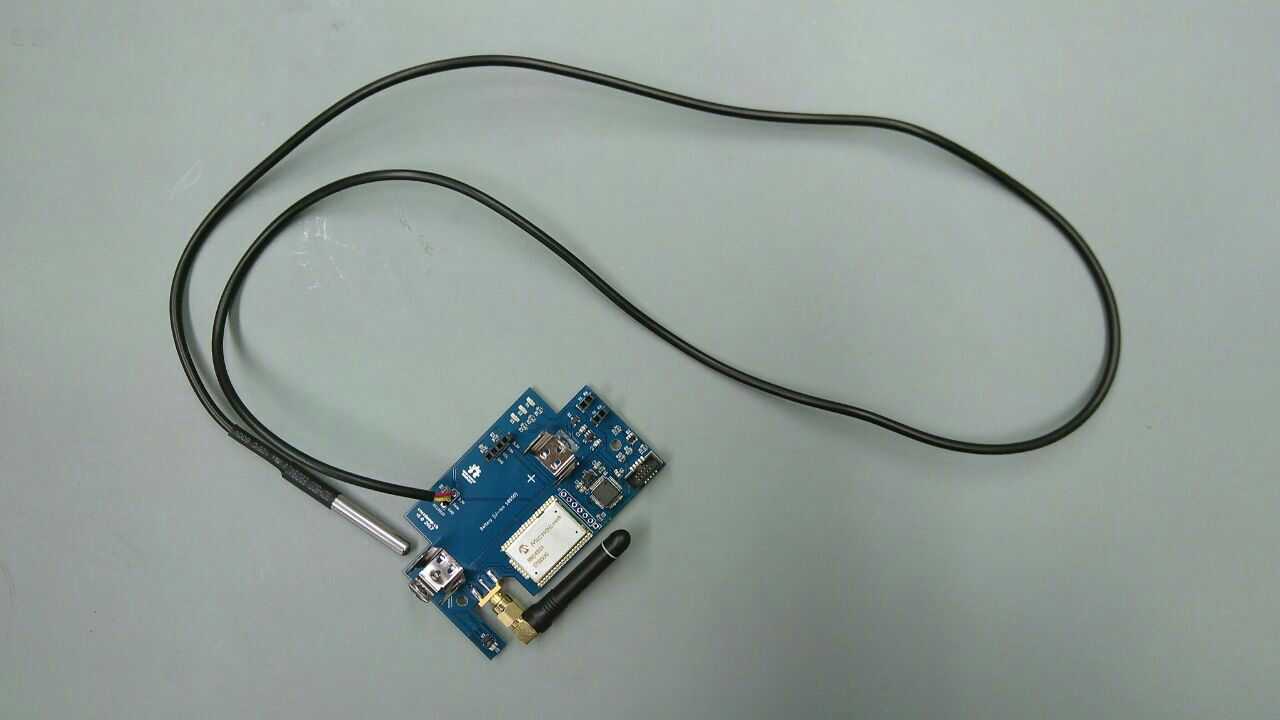
\includegraphics[width=.9\textwidth]{img/water-sensor-pcb.png}
\end{frame}

\begin{frame}[c]{water-sensor project}
  \begin{itemize}
    \item ``IoT'' project from coredump.ch
    \item µC, LoRaWAN modem, LEDs, I²C sensors
    \item Prototype runs with mbed C++
    \item<2-> But I had to much time at 34C3\ldots
  \end{itemize}
\end{frame}

\begin{frame}[c]{tuwat!}
  \centering
  
\includegraphics[width=.8\textwidth]{img/port-all-the-things.jpg}
\end{frame}

\begin{frame}[c]{cortex-m-quickstart}
  \ldots
\end{frame}

\section{Awesome Stuff}

\begin{frame}[c]{svd2rust}
  Compare C defines, C++ template magic, and svd2rust generated code
  Auto-completion could be awesome!
  No more typos or mixing up bit indices with values!
\end{frame}

\begin{frame}[c]{xargo}
\end{frame}

\section{Painful Stuff}

\begin{frame}[c]{Broken SVD files}
\end{frame}

\begin{frame}[c]{Breaking changes in nightly}
\end{frame}

\section{Future}

\begin{frame}[c]{Embedded Rust in 2018}
  Blogpost from jeparic?
\end{frame}

% ----------------------------------------------------------------- %

{
\setbeamertemplate{footline}{}
\pgfdeclareimage[width=\paperwidth]{bg}{background-inverted.pdf}
\usebackgroundtemplate{\pgfuseimage{bg}}
\begin{frame}[standout]
  \begin{centering}
    {\Huge Thank you!}\\
    {\normalsize \url{https://coredump.ch}}\\
  \end{centering}
  {\small Slides: \url{https://github.com/rust-zurichsee/meetups/}}\\
  \vspace{3cm}
\end{frame}
}
\end{document}
